\chapter{Scattering simulation}
\label{scattering}
Finally after all our hard work of investigating the dispersion curves of
different lattices as well as finding out how to perturb them such that we form
a bandgap, we will actually simulate how a wave of a certain frequency
propagates and scatters through a finite portion of one of our lattices.

Similarly to how we joined cells together to from a strip, we will do the same
and join strips to form a finite lattice. We may then reframe our eigen-problem
systems in reciprocal space into linear systems in physical space. From there,
we can solve the linear systems to see how the energy or wave moves throughout
the entire space. All we need to do is pick a frequency for the wave we want to
simulate as well as where we want the source of excitation to be.

From the dispersion relations, we know which frequency waves are able to
propagate across the lattice and which frequencies are not transmitted through
the lattice. As we have discussed before in Chapter \ref{formstrip}, we know
that there are certain frequencies which are only able to propagate along the
interface of the strips and not anywhere else in the lattice. These are the
frequencies which we will be simulating.

\section{Our linear system in physical space}
Before we can run our scattering simulations, which essentially is solving for
the displacements of masses in our finite lattice, we need to form the system
to solve. This actually turns out to be really similar to the eigen-problems we
had earlier (albeit with a much larger matrix involved!). It is also useful to
note that the following derivation works just as well for systems of any shape
as long as we have formed the eigen-problem as before, as we will reuse the
variables in the eigen-problem here.
 
We will show it for the hexagonal lattice. Looking at \eqref{eq:hexstripeig},
we first need to extend the system to include our whole finite lattice which is
formed by joining strips side-by-side. So now $\matr{A}$ is a $(2N \times M
\times 6) \times (2N \times M \times 6)$ matrix with $\matr{A}$ from
\eqref{eq:hexstripeig} repeated $M$ times along the diagonal, with the complex
exponential terms removed and additional coupling terms between masses in
adjacent strips added in. We also extend $\matr{M}$ by repeating $\matr{M}$ $M$
times along the diagonal.

The key idea now is just to notice that when we can pick and choose the
frequency, $\Omega$, the LHS
$\left[\matr{A}\left(\kappa_{x},\kappa_{y}\right)-\matr{\Omega}\matr{M}\right]=\matr{B}$
just falls out as a known-valued matrix. Then for the RHS, instead of
$\vec{0}$, we will have a vector $\vec{F}$ containing our forcing terms at the
masses which will act as our source of excitation, e.g. if we are inducing a
positive wave at the mass $M_i^{n,m}$, then we will have $\vec{F}$ is a vector
of $0$ except at the position which correpsonds to mass $M_i^{n,m}$ we will
have a $1$. Then we see

\begin{align}
  \matr{B}\vec{y}=\vec{F}
\end{align}

which is just a linear system we can solve for $\vec{y}$!

With this linear system set up, let us take a look at the physical spaces in
which we will run these simulations.

\section{2d hexagonal finite lattice}
\begin{figure}[!h]
\centering
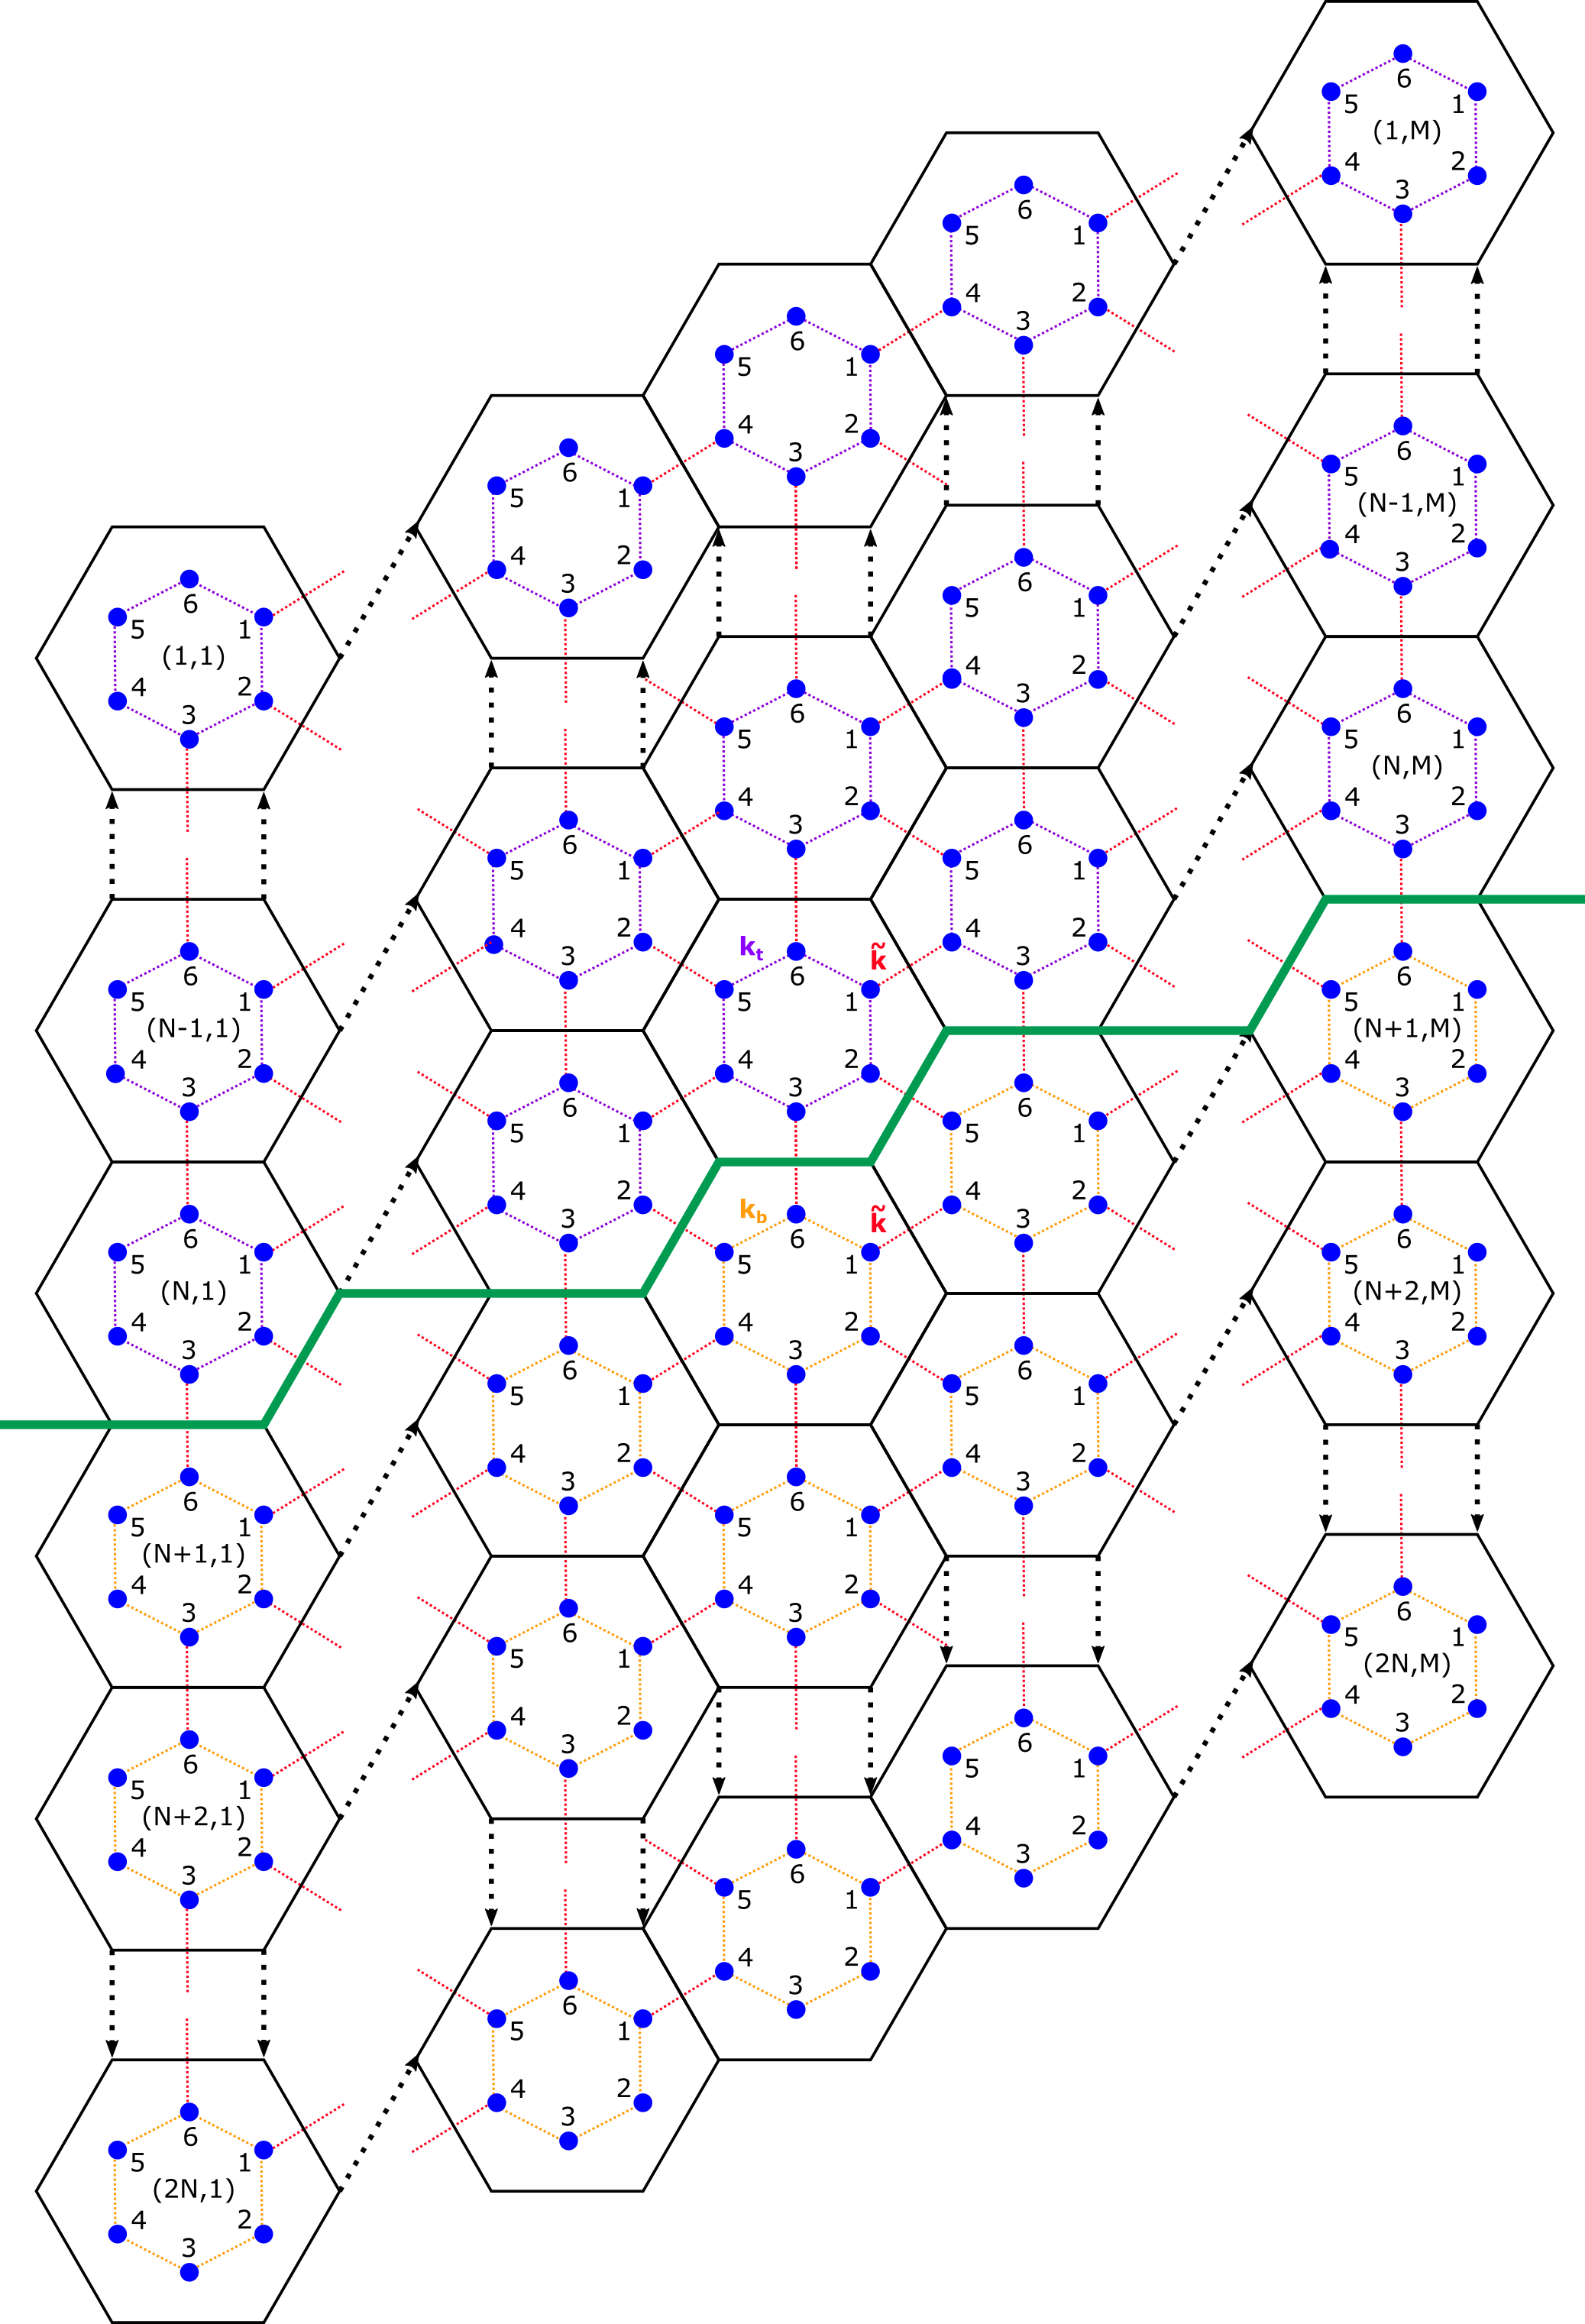
\includegraphics[width=0.8\textwidth]{imgs/hexfinitemodel.png}
\caption{\label{fig:hexfinscheme} Schematic view of the finite hexagonal
  lattice formed from the joining of strips side-by-side, where the strips
  themselves are formed from two different halves as in Chapter
  \ref{perturbed}. Note the conditions imposed at the boundaries (masses at
  boundaries have no connections outside the lattice).}
\end{figure}

Figure~\ref{fig:hexfinscheme} shows a schematic view of the finite hexagonal
lattice on which we are simulating our scattering. Specifically, we will be
running our following simulations on the arrangement of cells in
Figure~\ref{fig:hexstdfinlattice}. We will be exciting our lattice at the
leftmost edge of the boundary. More specifically, we will have a positive
excitation just above the boundary (at $M_4$), and a negative excitation just
below the boundary (at $M_5$), i.e. $\vec{F}$ is $0$ everywhere except
$\vec{F}_{6(\frac{N}{2}-1)+4}=1$ and $\vec{F}_{6(\frac{N}{2})+5}=-1$.

\begin{figure}[!h]
  \centering
  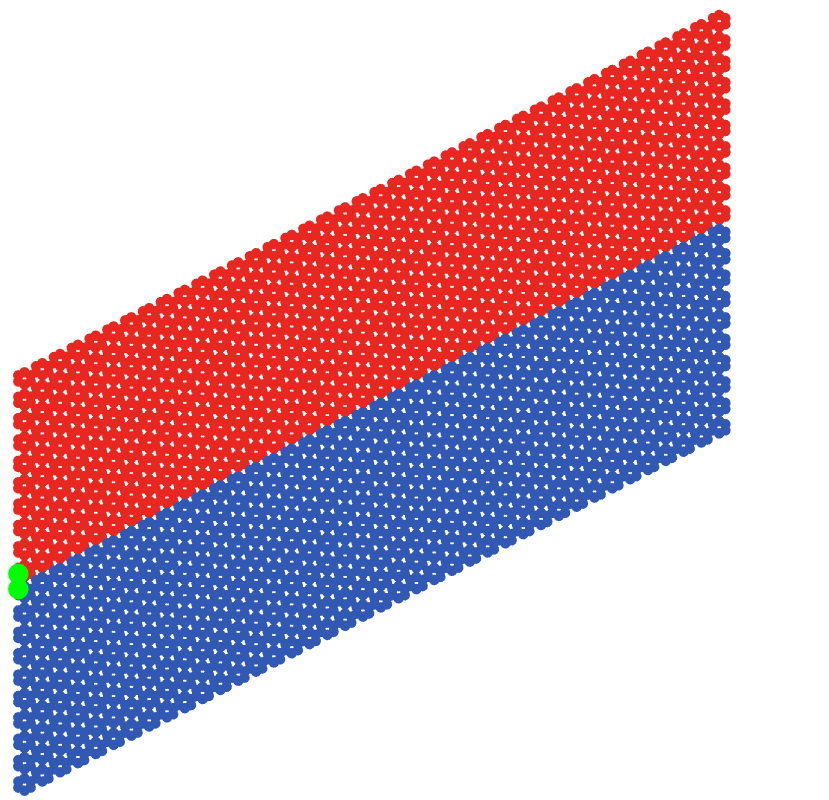
\includegraphics[width=0.5\linewidth]{imgs/hexstdfinlattice.png}
  \caption{Arrangement of hexagonal cells ($2N=20$, $M=40$), with red and blue
    being different materials, and source of excitation at the green masses.}
  \label{fig:hexstdfinlattice}
\end{figure}

\subsection{Alternating masses}

In this section we will run scattering simulations on the physical lattice as
described in Chapter \ref{perturbaltmass} with the alternating masses.

Now, we can run our simulations for another frequency we want, but we know from
our dispersion relations that most frequencies (those outside the special
dispersion curves corresponding to the edge states) will just propagate
throughout the lattice and so we would not get any discernible patterns of
movement. An example can be found in Figure~\ref{fig:randscat}.

\begin{figure}[!h]
\centering
\begin{subfigure}[b]{.5\textwidth}
  \centering
  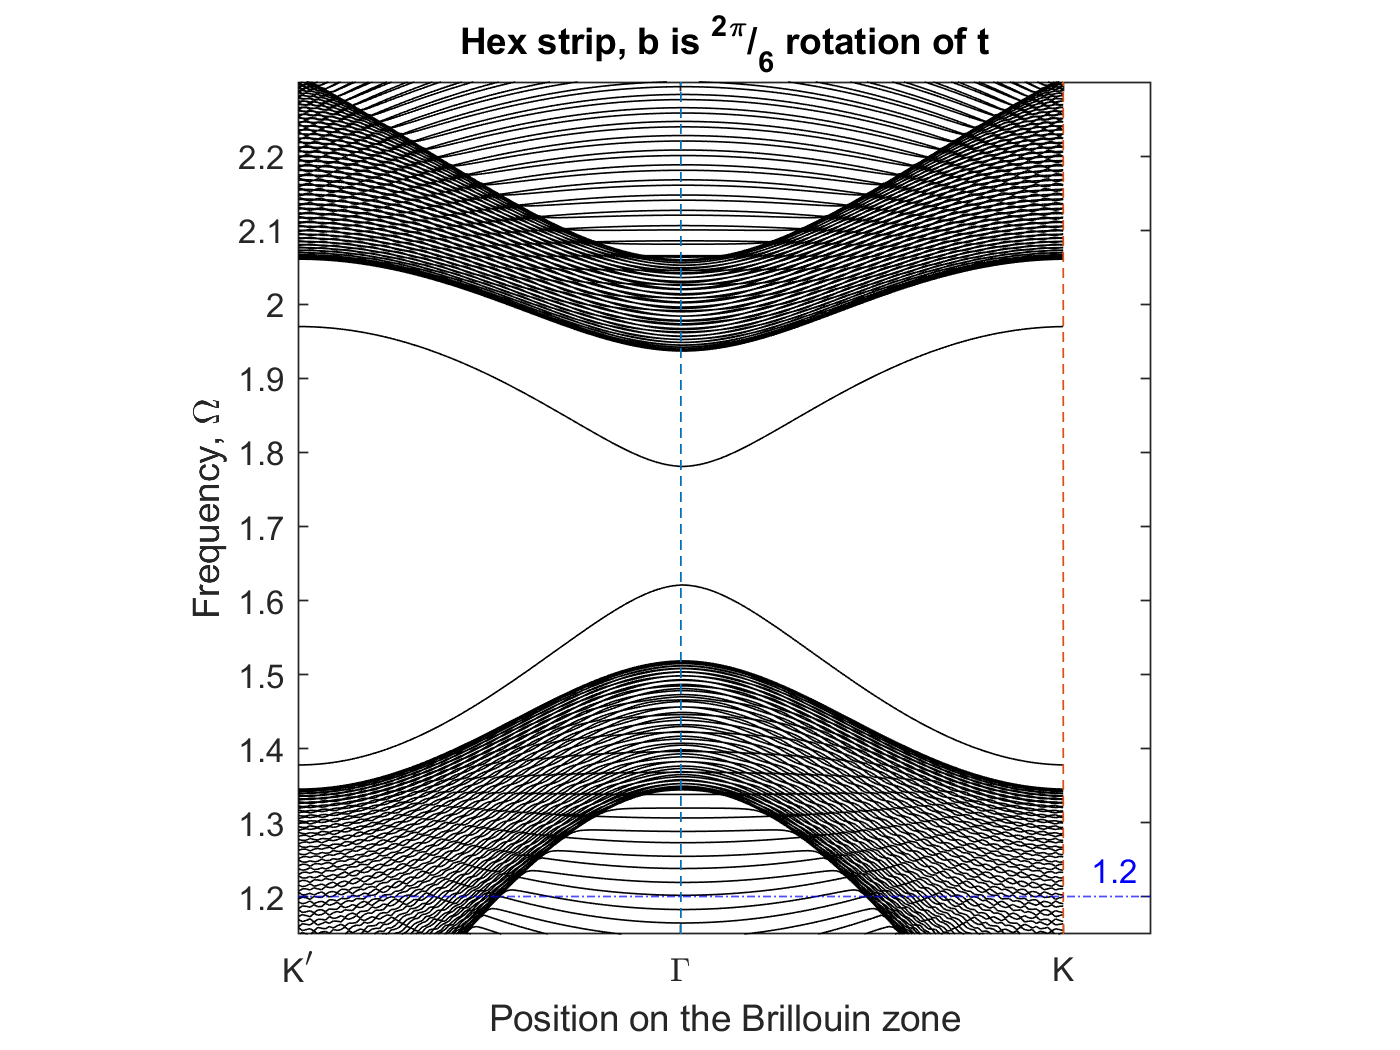
\includegraphics[width=1.1\linewidth]{imgs/hexstripperturbMrotatedrand.png}
  \caption{Zoomed in look of Figure~\ref{fig:hexstripMrotated} near the bandgap.}
\label{fig:sub1}
\end{subfigure}%
\begin{subfigure}[b]{.5\textwidth}
  \centering
  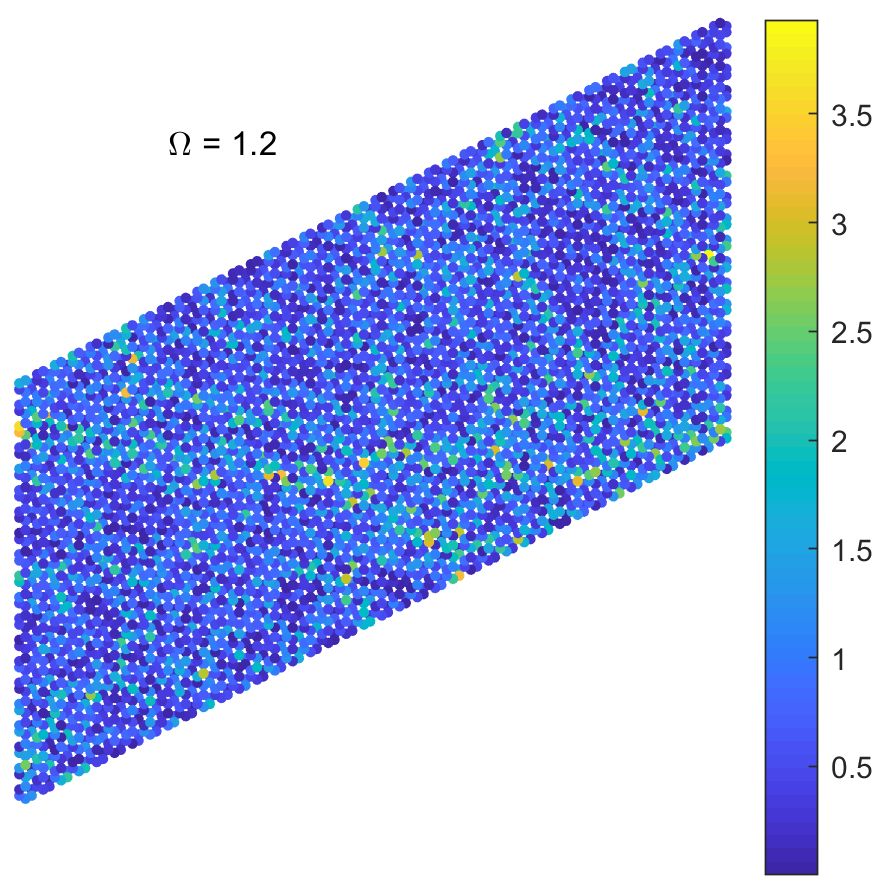
\includegraphics[width=1\linewidth]{imgs/hexstdrandscat.png}
  \caption{The plot of $|y_i|$ for each mass in each cell.}
  \label{fig:sub2}
\end{subfigure}
\caption{Simulation of scattering on the hexagonal finite lattice in
  Figure~\ref{fig:hexstdfinlattice} with the alternating masses as defined in
  Figure~\ref{fig:hexstripMrotated} with $\Omega = 1.2$.}
\label{fig:randscat}
\end{figure}

As we are interested in being able to direct waves to our liking, it is much
more exciting to fire a frequency which is only able to travel along the
boundary. So let use the same system as in Figure~\ref{fig:randscat} again, but
using $\Omega = 1.6$ instead as we can see in
Figure~\ref{fig:hexstripMrotatedzooms1} that the dispersion curve for that edge
mode lives in the bandgap.

\begin{figure}[!h]
\centering
\begin{subfigure}[b]{.5\textwidth}
  \centering
  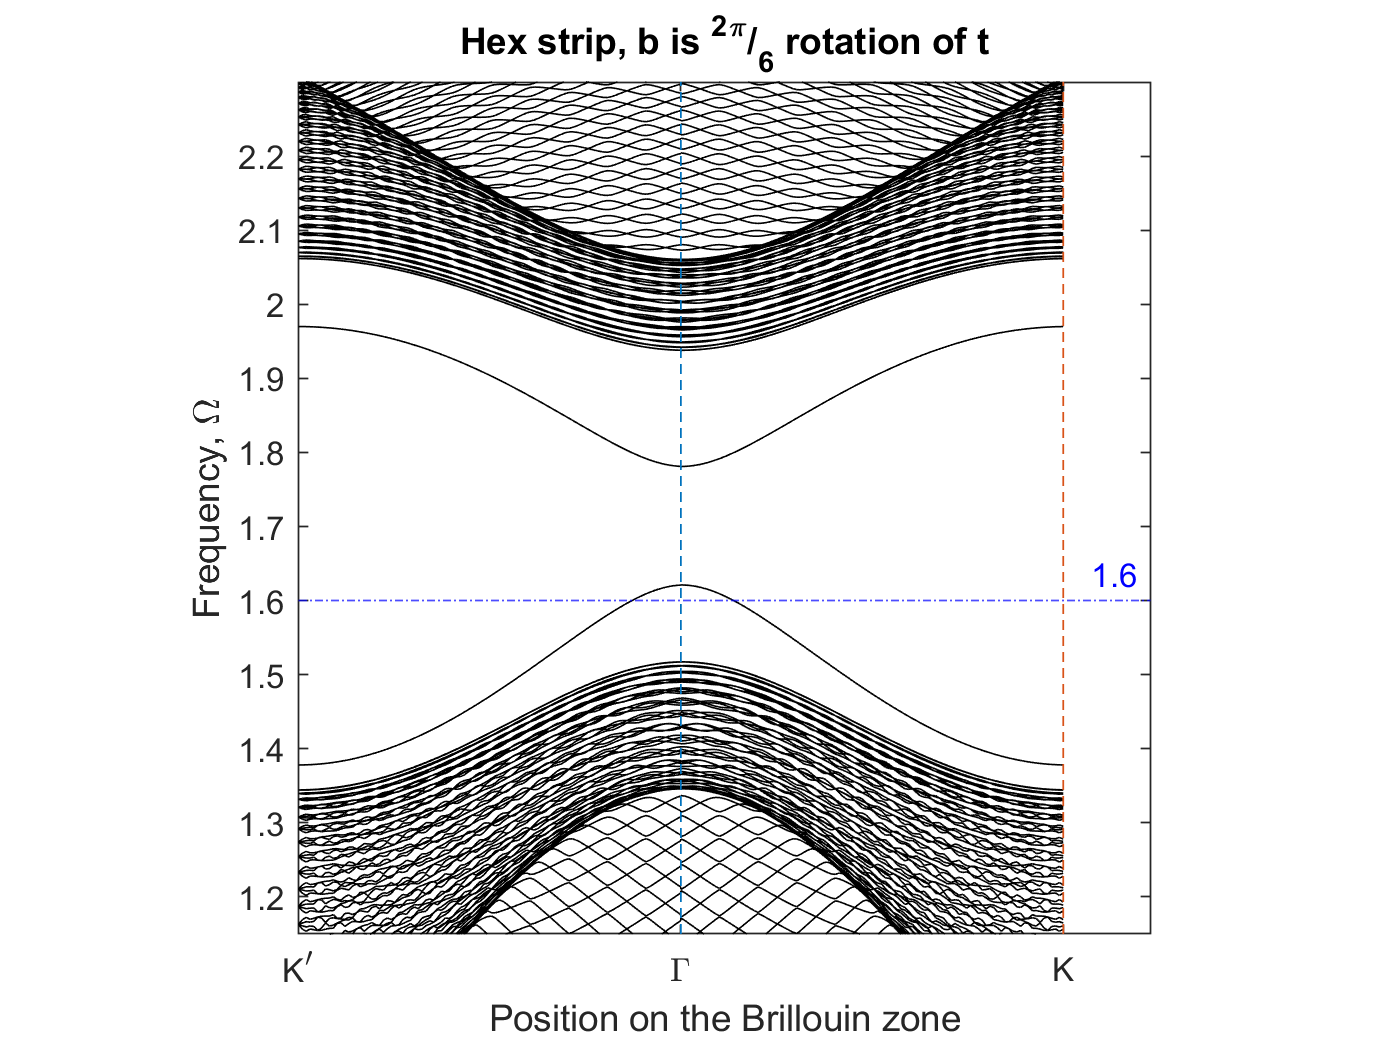
\includegraphics[width=1.1\linewidth]{imgs/hexstripperturbMrotatedzoom.png}
  \caption{Zoomed in look of Figure~\ref{fig:hexstripMrotated} near the bandgap.}
  \label{fig:hexstripMrotatedzooms1}
\end{subfigure}%
\begin{subfigure}[b]{.5\textwidth}
  \centering
  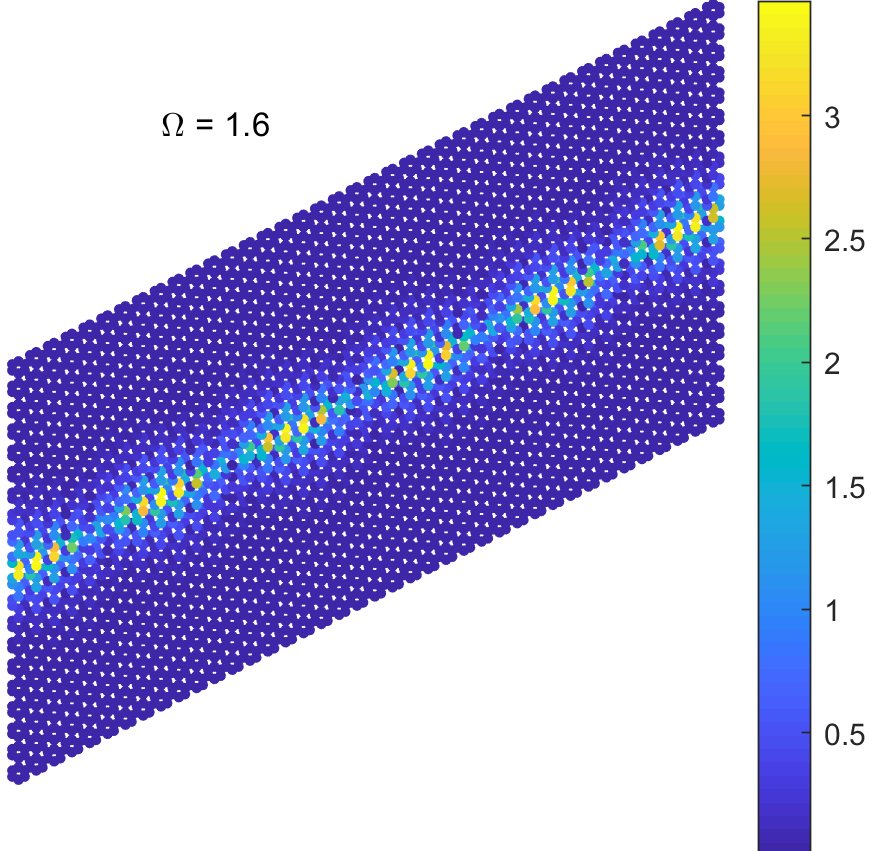
\includegraphics[width=1\linewidth]{imgs/hexstdrotstraight.png}
  \caption{The plot of $|y_i|$ for each mass in each cell.}
  \label{fig:sub2}
\end{subfigure}
\caption{Simulation of scattering on the hexagonal finite lattice in
  Figure~\ref{fig:hexstdfinlattice} with the alternating masses as defined in
  Figure~\ref{fig:hexstripMrotated} with $\Omega = 1.6$.}
\label{fig:hexstdrotstraight}
\end{figure}

Wonderful! Finally after all our hard work we can see in
Figure~\ref{fig:hexstdrotstraight} that the wave or energy forced into the
system is only propagating along the straight line. This effectively means that
we can control the direction of propagation of waves through our lattice and
not have it diffuse or \textit{leak} out into the other parts of the lattice.
Of course our next thought would be to see if it is possible to send the energy
around bends and more complex boundaries, which is what we discuss in Chapter
\ref{complexbends}.

\subsection{Varying mass and stiffnesses}
Now we take a look at running scattering simulations as above but for the
physical system discussed in Chapter \ref{perturbMk}, which results in
Figure~\ref{hexstdMk}.

\begin{figure}[!h]
\centering
\begin{subfigure}[b]{.5\textwidth}
  \centering
  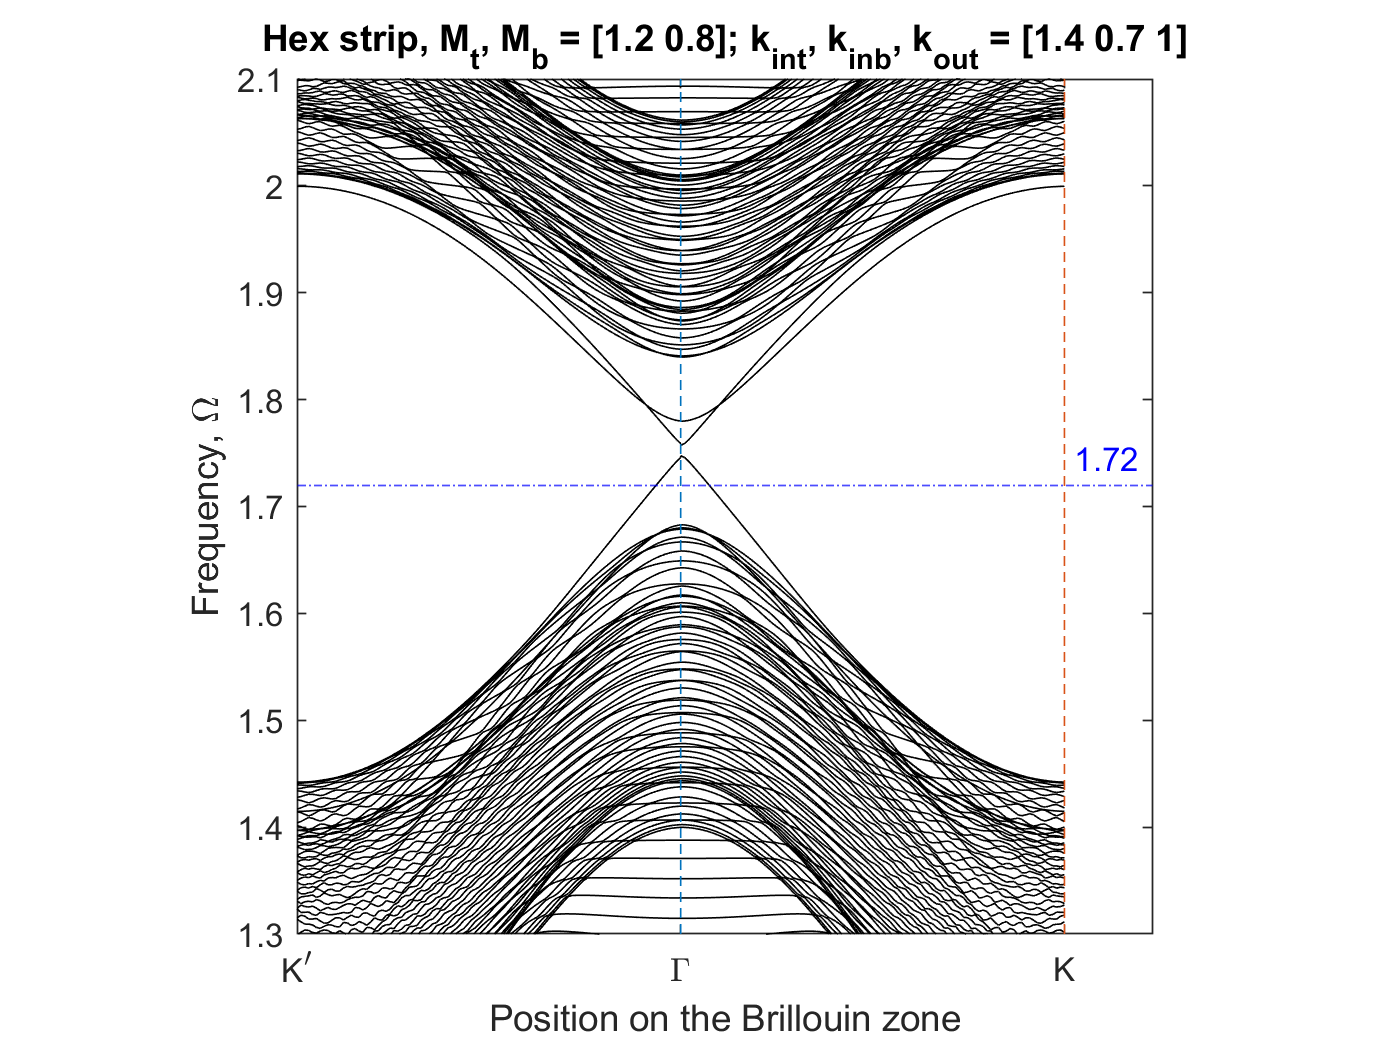
\includegraphics[width=1.1\linewidth]{imgs/hexstripperturb2zoom.png}
  \caption{Zoomed in look of Figure~\ref{fig:hexstrip2} near the bandgap.}
  \label{fig:sub1}
\end{subfigure}%
\begin{subfigure}[b]{.5\textwidth}
  \centering
  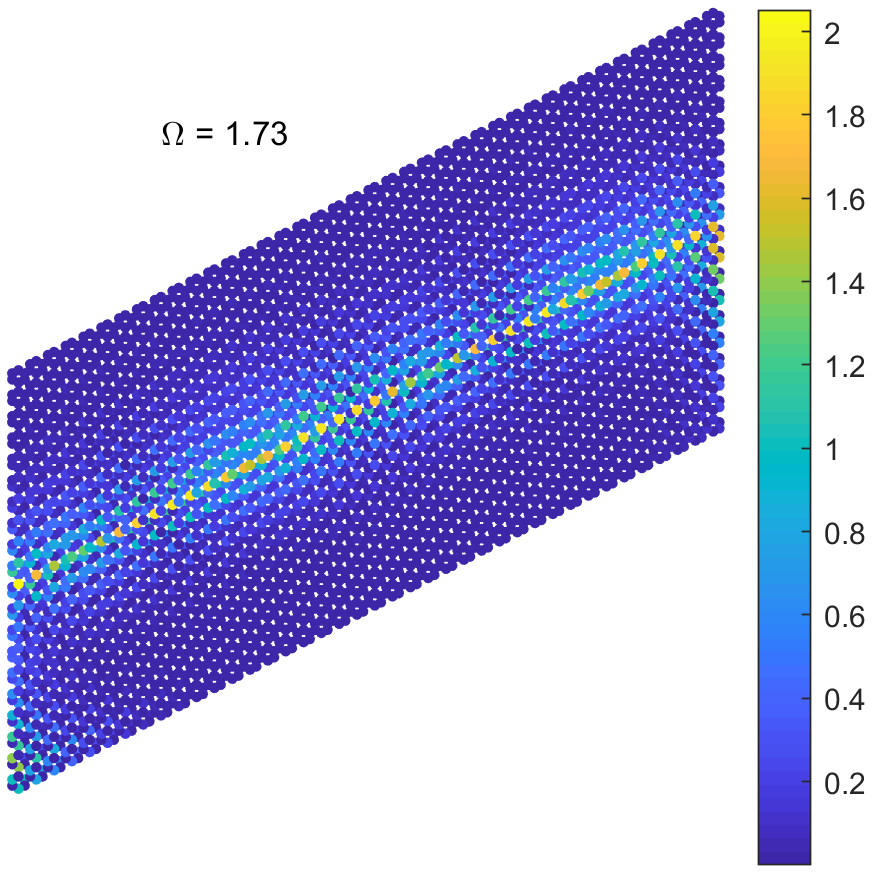
\includegraphics[width=1\linewidth]{imgs/hexstdMk.png}
  \caption{The plot of $|y_i|$ for each mass in each cell.}
  \label{fig:sub2}
\end{subfigure}
\caption{Simulation of scattering on the hexagonal finite lattice in
  Figure~\ref{fig:hexstdfinlattice} with the top having a greater $M$ and $k$
  than the bottom as defined in Figure~\ref{fig:hexstrip2} with $\Omega =
  1.72$.}
\label{fig:hexstdMk}
\end{figure}

\section{2d kagome finite lattice}
\begin{figure}[!h]
\centering
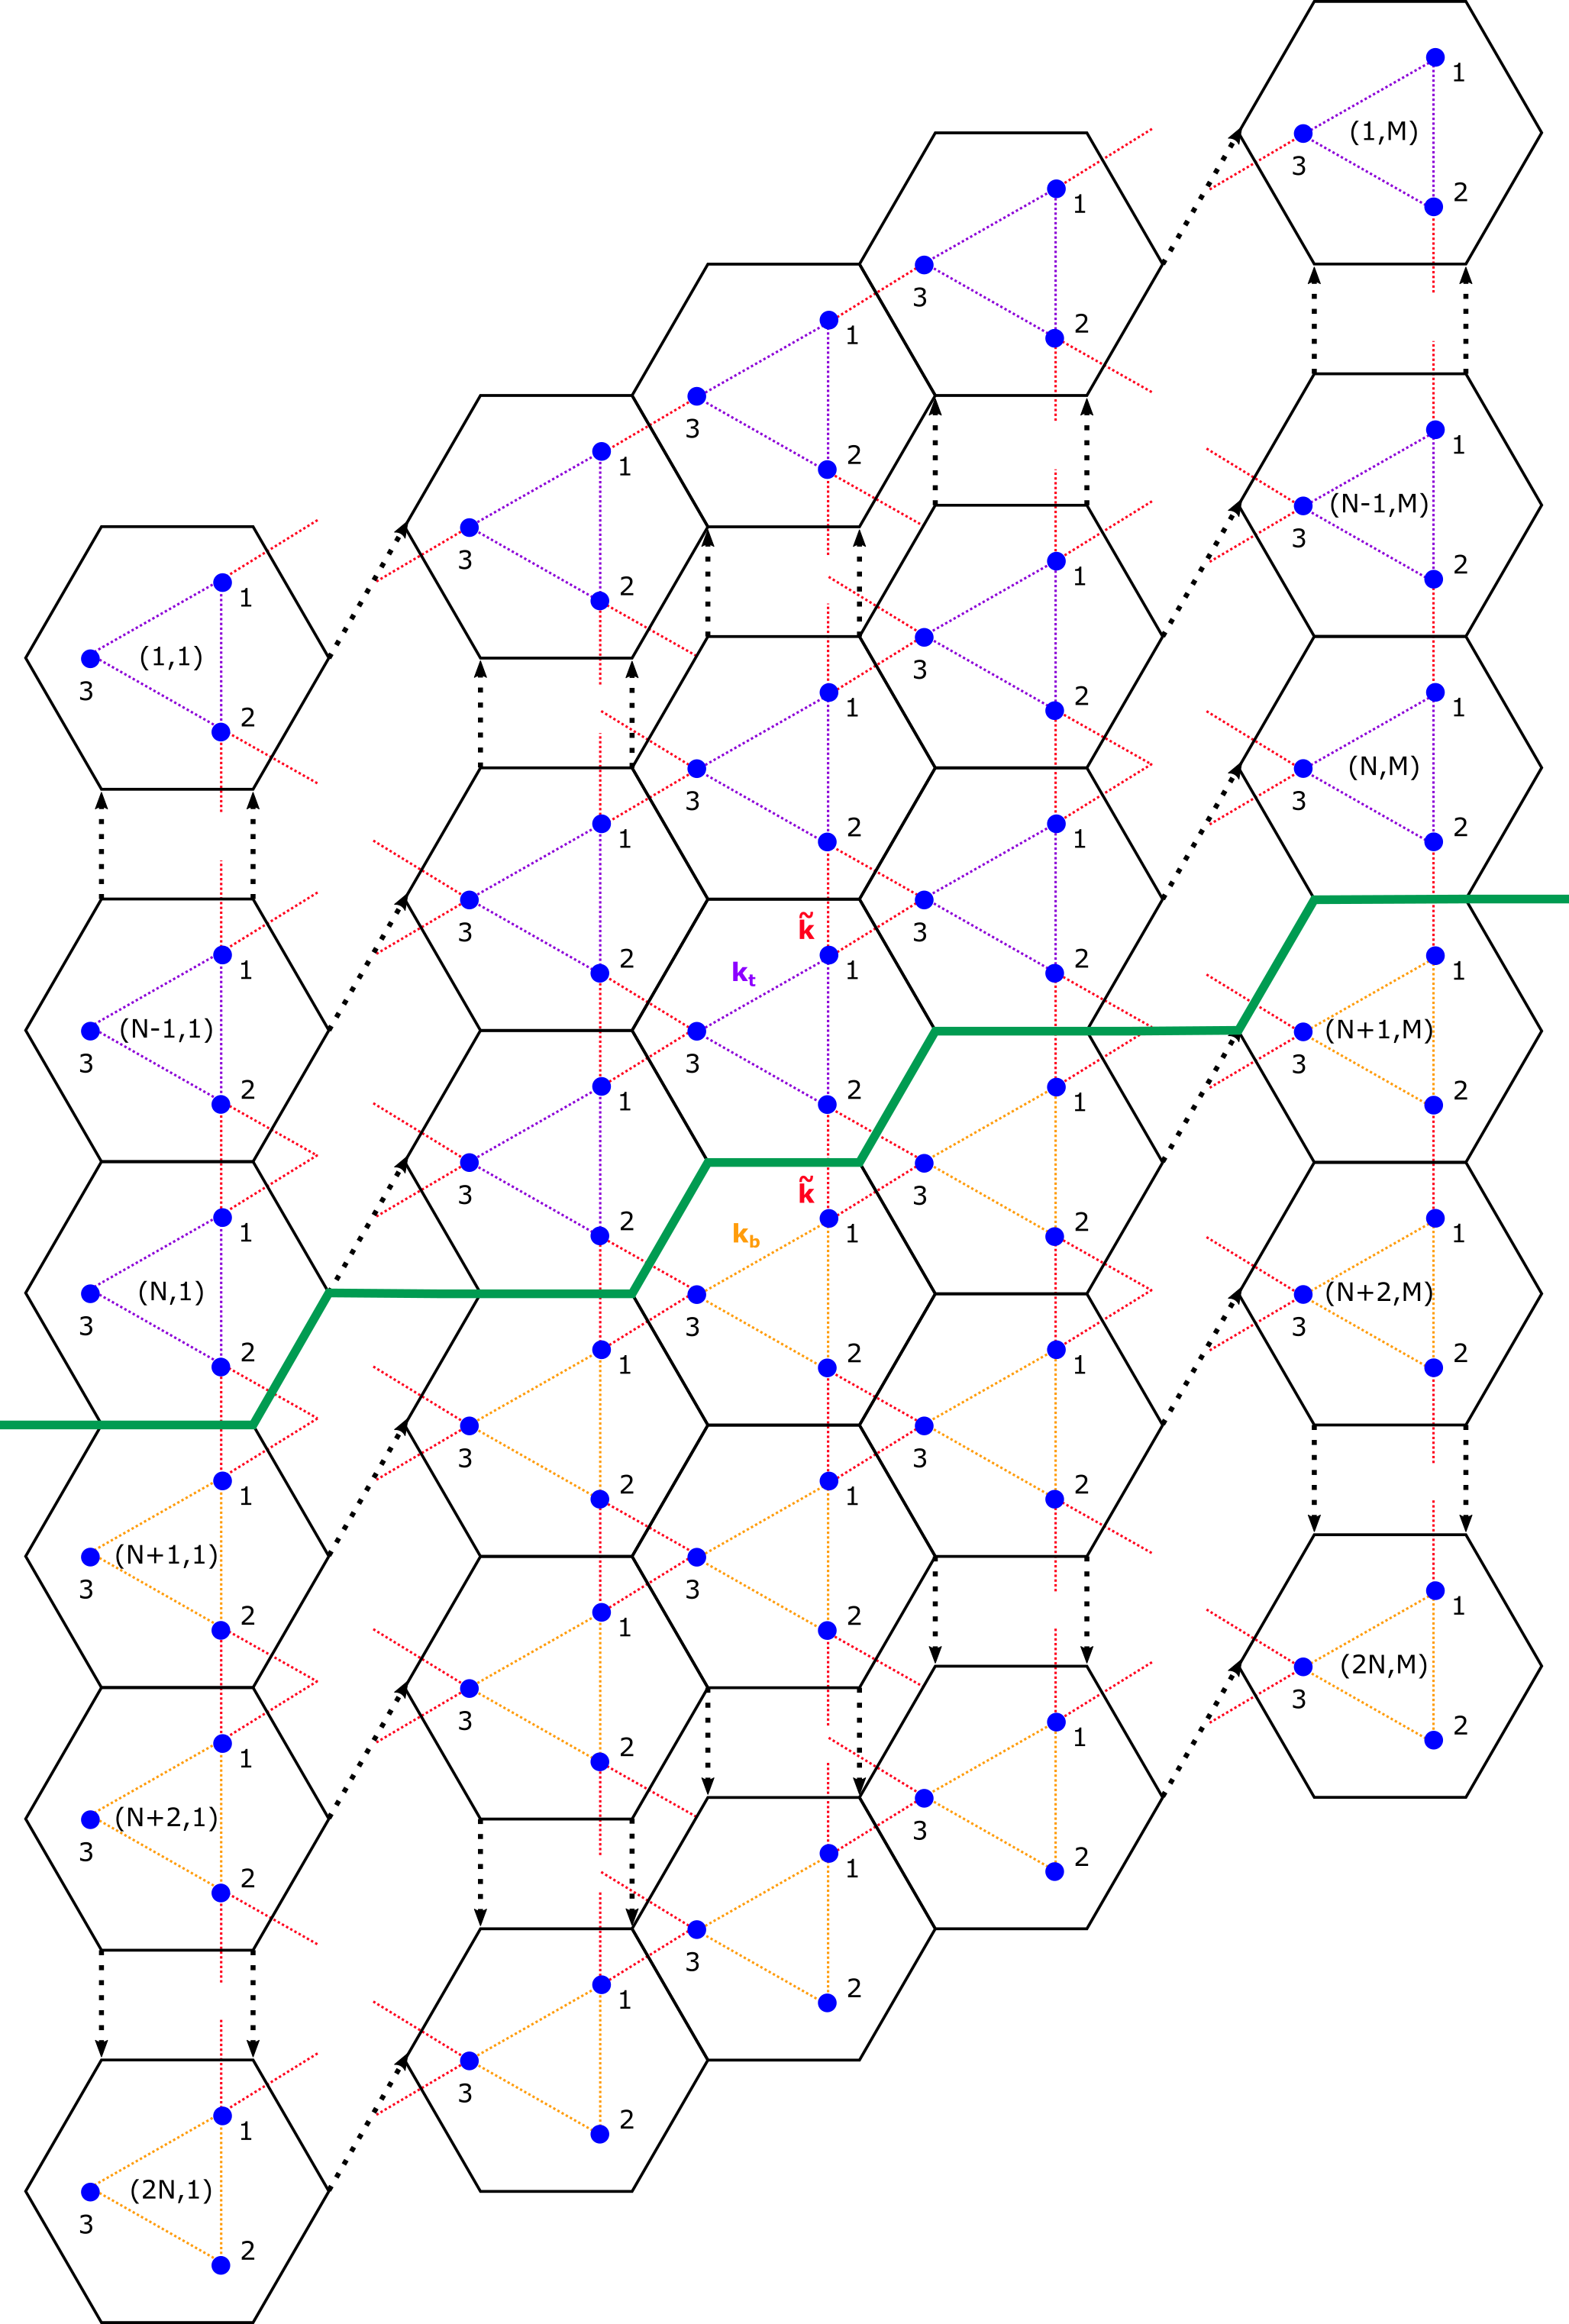
\includegraphics[width=0.8\textwidth]{imgs/kagomefinitemodel.png}
\caption{\label{fig:kagomefinscheme} Schematic view of the finite kagome
  lattice formed from the joining of strips side-by-side, where the strips
  themselves are formed from two different halves as in Chapter
  \ref{perturbed}. Note the conditions imposed at the boundaries (masses at
  boundaries have no connections outside the lattice).}
\end{figure}

Figure~\ref{fig:kagomefinscheme} shows a schematic view of the finite kagome
lattice on which we will be running our scattering simulations. We will be
exciting our lattice at the leftmost edge of the boundary. More specifically,
we will have a positive excitation just above the boundary (at $M_3$), and a
negative excitation just below the boundary (at $M_3$), i.e. $\vec{F}$ is $0$
everywhere except $\vec{F}_{3(\frac{N}{2}-1)+3}=1$ and
$\vec{F}_{3(\frac{N}{2})+3}=-1$.

\medskip
Running our simulation on the arrangement of cells in
Figure~\ref{fig:kagomestdfinlattice}, we get the edge state in
Figure~\ref{fig:kagomestd}. The only difference between this and the hexagonal
ones is that we can see there seems to be some of the energy being diverted
down the right edge. This is due to the way we have set up the boundary
conditions in which we have rigid boundaries. This boundary coinciding with the
straight line connections of $M_1$ connected to $M_2$ allows certain waves to
be trasmitted along that boundary. Something very similar happens along the top
boundary where there is a straight line connection between $M_1$ and $M_3$,
which we can see in Figure~\ref{fig:kagomegentlebendscat}.

\begin{figure}[!h]
  \centering
  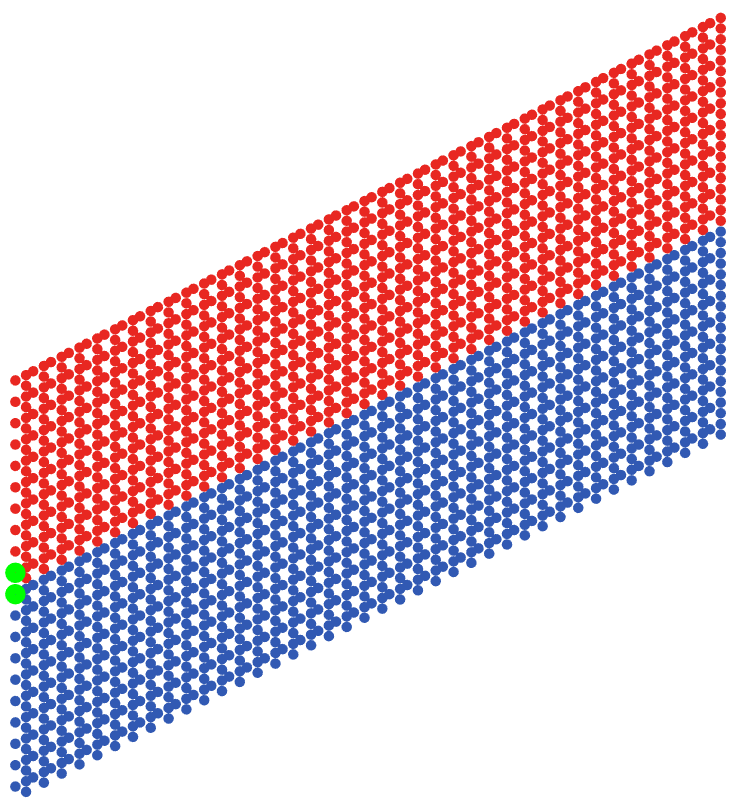
\includegraphics[width=0.5\linewidth]{imgs/kagomestdarr.png}
  \caption{Arrangement of kagome cells ($2N=20$, $M=40$), with red and blue
    being different materials, and source of excitation at the green masses.}
  \label{fig:kagomestdfinlattice}
\end{figure}

\begin{figure}[!h]
\centering
\begin{subfigure}[b]{.5\textwidth}
  \centering
  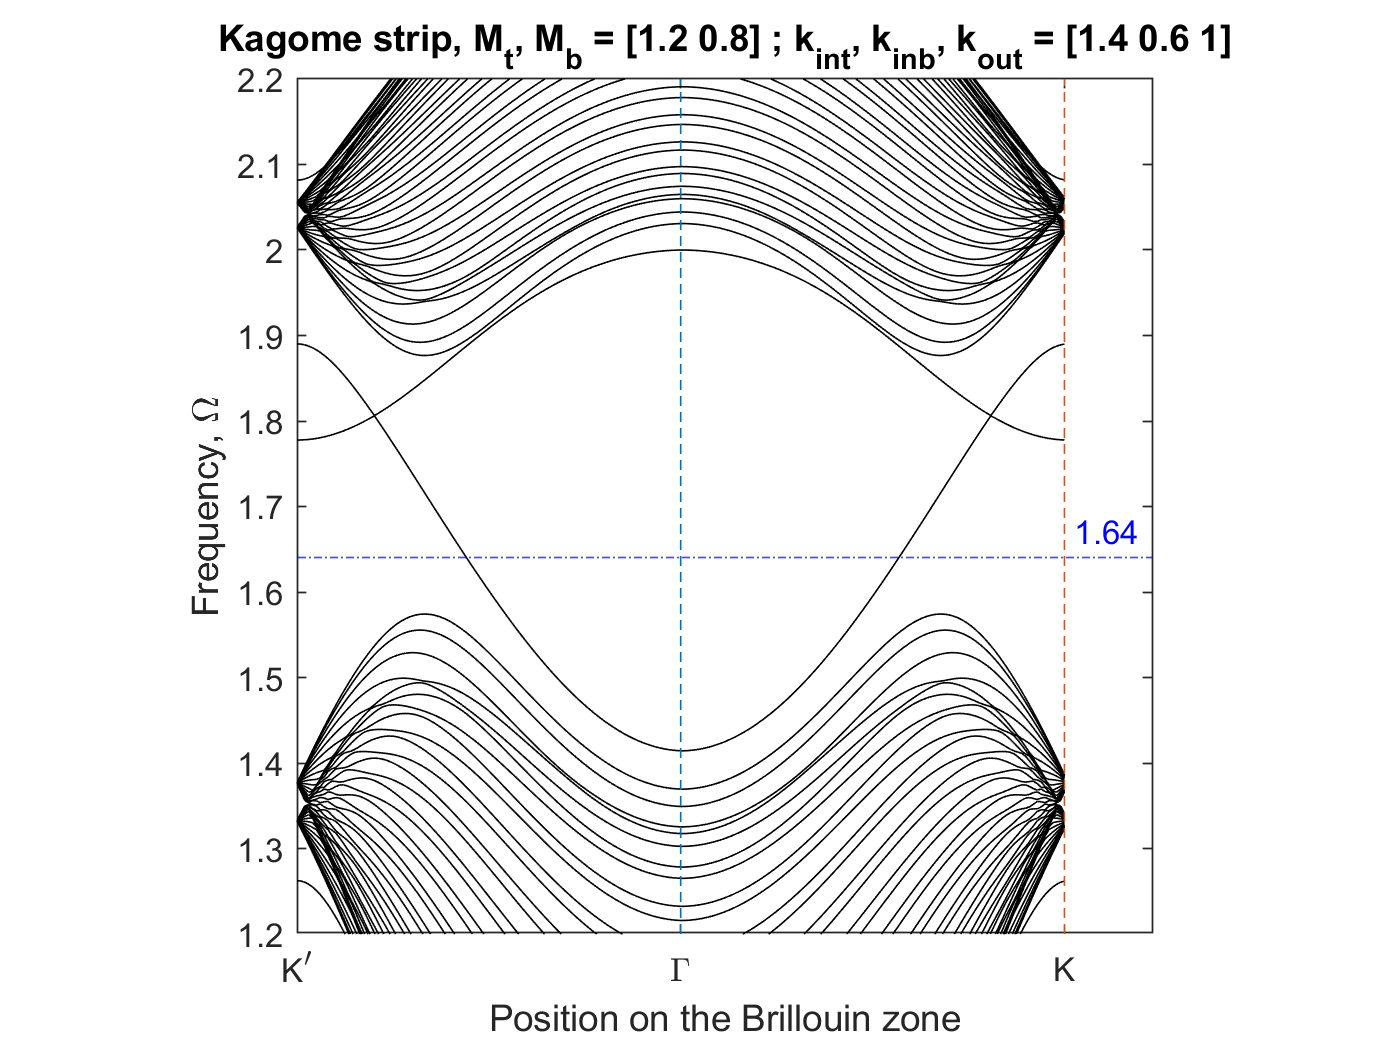
\includegraphics[width=1.1\linewidth]{imgs/kagomeperturb2zoom.png}
  \caption{Zoomed in look of Figure~\ref{fig:kagomeperturbed} near the bandgap.}
  \label{fig:sub1}
\end{subfigure}%
\begin{subfigure}[b]{.5\textwidth}
  \centering
  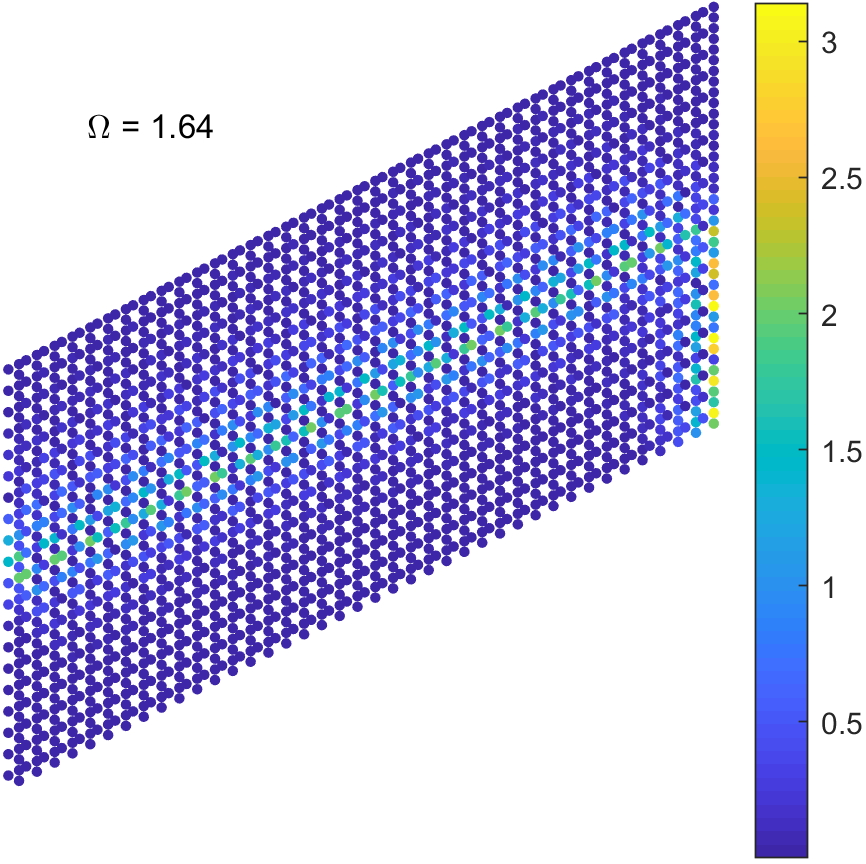
\includegraphics[width=1\linewidth]{imgs/kagomestd.png}
  \caption{The plot of $|y_i|$ for each mass in each cell.}
  \label{fig:sub2}
\end{subfigure}
\caption{Simulation of scattering on the kagome finite lattice in
  Figure~\ref{fig:kagomestdfinlattice} with the top material with greater $M$
  and $k$ than the bottom material as defined in
  Figure~\ref{fig:kagomeperturbed} with $\Omega = 1.64$.}
\label{fig:kagomestd}
\end{figure}
